% =============================================================================
% Episode 024: Lessons Learned and Best Practices
% Series: DIP-SMC-PSO Professional Toolkit
% Phase: 4 (Appendix & Reference)
% Duration: ~20 minutes | Pages: 8-10 | Complexity: Reference
% Dependencies: All phases (6-month retrospective)
% =============================================================================

% ==============================================================================
% MASTER TEMPLATE FOR PODCAST EPISODE CHEATSHEET PDFs
% ==============================================================================
% Purpose: Beginner-friendly, colorful, multi-page study guides (2-4 pages)
% Target Audience: Complete beginners (Path 0 learners)
% Visual Style: Infographic-style with vibrant colors, icons, callout boxes
% ==============================================================================

\documentclass[11pt,a4paper]{article}

% ------------------------------------------------------------------------------
% GEOMETRY & LAYOUT
% ------------------------------------------------------------------------------
\usepackage[top=1.5cm, bottom=1.5cm, left=1.5cm, right=1.5cm, headheight=14pt]{geometry}
\usepackage{multicol}
\usepackage{fancyhdr}
\pagestyle{fancy}

% ------------------------------------------------------------------------------
% COLOR PALETTE (Vibrant & Beginner-Friendly)
% ------------------------------------------------------------------------------
\usepackage{xcolor}
\definecolor{primary}{RGB}{41, 128, 185}      % Blue - Main concepts, headers
\definecolor{secondary}{RGB}{39, 174, 96}     % Green - Success, examples
\definecolor{accent}{RGB}{230, 126, 34}       % Orange - Important notes
\definecolor{warning}{RGB}{231, 76, 60}       % Red - Common pitfalls
\definecolor{background}{RGB}{236, 240, 241}  % Light gray - Callout boxes
\definecolor{codeblock}{RGB}{44, 62, 80}      % Dark blue-gray - Code background
\definecolor{highlight}{RGB}{241, 196, 15}    % Yellow - Highlights

% ------------------------------------------------------------------------------
% TIKZ & GRAPHICS
% ------------------------------------------------------------------------------
\usepackage{tikz}
\usetikzlibrary{shapes, arrows, positioning, calc, shadows, decorations.pathreplacing, backgrounds, fit}
\usepackage{graphicx}
\usepackage{float}

% TikZ styles for consistent diagrams
\tikzstyle{block} = [rectangle, draw, fill=primary!20, text width=5em, text centered, rounded corners, minimum height=3em, drop shadow]
\tikzstyle{arrow} = [thick,->,>=stealth]
\tikzstyle{process} = [rectangle, draw, fill=secondary!20, text width=6em, text centered, rounded corners, minimum height=3em]
\tikzstyle{decision} = [diamond, draw, fill=accent!20, text width=4.5em, text badly centered, inner sep=0pt]
\tikzstyle{cloud} = [ellipse, draw, fill=background, text width=5em, text centered, minimum height=2.5em]

% ------------------------------------------------------------------------------
% BOXES & CALLOUTS (tcolorbox)
% ------------------------------------------------------------------------------
\usepackage{tcolorbox}
\tcbuselibrary{skins, breakable, raster}

% Key Concept Box (Blue)
\newtcolorbox{keypoint}{
    enhanced,
    colback=primary!10,
    colframe=primary,
    fonttitle=\bfseries,
    title=\faLightbulb\ Key Concept,
    attach boxed title to top left={yshift=-2mm, xshift=5mm},
    boxed title style={colback=primary},
    breakable
}

% Example Box (Green)
\newtcolorbox{example}{
    enhanced,
    colback=secondary!10,
    colframe=secondary,
    fonttitle=\bfseries,
    title=\faCode\ Example,
    attach boxed title to top left={yshift=-2mm, xshift=5mm},
    boxed title style={colback=secondary},
    breakable
}

% Warning Box (Red)
\newtcolorbox{warning}{
    enhanced,
    colback=warning!10,
    colframe=warning,
    fonttitle=\bfseries,
    title=\faExclamationTriangle\ Common Pitfall,
    attach boxed title to top left={yshift=-2mm, xshift=5mm},
    boxed title style={colback=warning},
    breakable
}

% Tip Box (Orange)
\newtcolorbox{tip}{
    enhanced,
    colback=accent!10,
    colframe=accent,
    fonttitle=\bfseries,
    title=\faLightbulb\ Pro Tip,
    attach boxed title to top left={yshift=-2mm, xshift=5mm},
    boxed title style={colback=accent},
    breakable
}

% Summary Box (Light gray)
\newtcolorbox{summary}{
    enhanced,
    colback=background,
    colframe=codeblock,
    fonttitle=\bfseries,
    title=\faListUl\ Quick Summary,
    attach boxed title to top left={yshift=-2mm, xshift=5mm},
    boxed title style={colback=codeblock},
    breakable
}

% ------------------------------------------------------------------------------
% ICONS & SYMBOLS (fontawesome5)
% ------------------------------------------------------------------------------
\usepackage{fontawesome5}

% Custom icon commands for consistency
\newcommand{\iconKey}{\textcolor{primary}{\faLightbulb}}
\newcommand{\iconCode}{\textcolor{secondary}{\faCode}}
\newcommand{\iconWarning}{\textcolor{warning}{\faExclamationTriangle}}
\newcommand{\iconTip}{\textcolor{accent}{\faInfoCircle}}
\newcommand{\iconLink}{\textcolor{primary}{\faLink}}
\newcommand{\iconBook}{\textcolor{secondary}{\faBook}}
\newcommand{\iconTarget}{\textcolor{accent}{\faBullseye}}

% ------------------------------------------------------------------------------
% TYPOGRAPHY & FONTS
% ------------------------------------------------------------------------------
\usepackage{lmodern}
\usepackage[T1]{fontenc}
\usepackage[utf8]{inputenc}

% Section styling
\usepackage{titlesec}
\titleformat{\section}{\Large\bfseries\color{primary}}{\thesection}{1em}{}[\titlerule]
\titleformat{\subsection}{\large\bfseries\color{secondary}}{\thesubsection}{1em}{}

% ------------------------------------------------------------------------------
% CODE LISTINGS
% ------------------------------------------------------------------------------
\usepackage{listings}
\lstset{
    basicstyle=\ttfamily\footnotesize\color{white},
    backgroundcolor=\color{codeblock},
    keywordstyle=\color{primary!80},
    commentstyle=\color{secondary!60}\itshape,
    stringstyle=\color{accent!80},
    numbers=left,
    numberstyle=\tiny\color{white!50},
    stepnumber=1,
    numbersep=8pt,
    frame=single,
    rulecolor=\color{codeblock},
    breaklines=true,
    breakatwhitespace=true,
    tabsize=4,
    captionpos=b
}

% Python-specific styling
\lstdefinestyle{python}{
    language=Python,
    morekeywords={self, def, class, import, from, as, return, if, else, elif, for, while, True, False, None}
}

% YAML-specific styling
\lstdefinestyle{yaml}{
    basicstyle=\ttfamily\footnotesize,
    showstringspaces=false,
    commentstyle=\color{secondary!60}\itshape,
    keywordstyle=\color{primary!80}
}

% ------------------------------------------------------------------------------
% HYPERLINKS
% ------------------------------------------------------------------------------
\usepackage{hyperref}
\hypersetup{
    colorlinks=true,
    linkcolor=primary,
    urlcolor=secondary,
    citecolor=accent
}

% ------------------------------------------------------------------------------
% HEADER & FOOTER CUSTOMIZATION
% ------------------------------------------------------------------------------
\fancyhf{}
\fancyhead[L]{\textcolor{primary}{\textbf{DIP-SMC-PSO Podcast Cheatsheet}}}
\fancyhead[R]{\textcolor{secondary}{\episodetitle}}
\fancyfoot[C]{\textcolor{primary}{\thepage}}
\renewcommand{\headrulewidth}{0.5pt}
\renewcommand{\footrulewidth}{0.5pt}

% ------------------------------------------------------------------------------
% CUSTOM COMMANDS
% ------------------------------------------------------------------------------

% Episode title command (to be defined in each episode file)
\newcommand{\episodetitle}{Episode Title}

% Learning objective command
\newcommand{\learningobjective}[1]{%
    \begin{center}
    \begin{tcolorbox}[colback=highlight!30, colframe=accent, width=0.9\textwidth]
    \iconTarget\ \textbf{Learning Objective:} #1
    \end{tcolorbox}
    \end{center}
}

% Quick reference command (for formulas/code snippets)
\newcommand{\quickref}[2]{%
    \begin{tcolorbox}[colback=background, colframe=primary, title=\faBookmark\ #1]
    #2
    \end{tcolorbox}
}

% Resource link command
\newcommand{\resourcelink}[2]{%
    \iconLink\ \href{#1}{\textcolor{secondary}{#2}}
}

% ------------------------------------------------------------------------------
% TITLE PAGE FORMATTING
% ------------------------------------------------------------------------------
\usepackage{afterpage}

\newcommand{\makeepisodetitle}[4]{%
    \begin{titlepage}
    \begin{tikzpicture}[remember picture, overlay]
        % Background gradient
        \fill[primary!20] (current page.south west) rectangle (current page.north east);

        % Title box
        \node[
            fill=white,
            rounded corners=10pt,
            drop shadow,
            text width=0.8\paperwidth,
            align=center
        ] at (current page.center) {
            \Huge\bfseries\color{primary} #1 \\[1em]
            \Large\color{secondary} #2 \\[2em]
            \large\color{codeblock} Part #3 $\cdot$ Duration: #4 \\[1em]
            \normalsize\color{codeblock} \textit{Beginner-Friendly Visual Study Guide}
        };

        % Footer
        \node[
            anchor=south,
            text width=0.9\paperwidth,
            align=center
        ] at (current page.south) {
            \color{primary}\rule{0.8\paperwidth}{0.5pt} \\[0.5em]
            \small\color{codeblock}
            \textbf{Repository:} \url{https://github.com/theSadeQ/dip-smc-pso} \\
            \textbf{Documentation:} academic/paper/presentations/podcasts/episodes/ \\[1em]
        };
    \end{tikzpicture}
    \end{titlepage}
}

% ------------------------------------------------------------------------------
% MATH & EQUATIONS
% ------------------------------------------------------------------------------
\usepackage{amsmath, amssymb, amsthm}
\usepackage{mathtools}

% Equation box (highlighted equations)
\newcommand{\eqbox}[1]{%
    \begin{tcolorbox}[colback=primary!5, colframe=primary, boxrule=1pt]
    \begin{equation}
    #1
    \end{equation}
    \end{tcolorbox}
}

% ------------------------------------------------------------------------------
% TABLES
% ------------------------------------------------------------------------------
\usepackage{booktabs}
\usepackage{array}
\usepackage{multirow}
\usepackage{colortbl}

% Custom table colors
\newcommand{\tableheadcolor}{\rowcolor{primary!30}}

% ------------------------------------------------------------------------------
% END OF PREAMBLE
% ------------------------------------------------------------------------------


% Episode Metadata
\title{\textbf{E024: Lessons Learned}}
\def\episodenumber{024}
\def\episodetitle{Lessons Learned \& Best Practices}
\def\episodecategory{Appendix \& Reference}
\def\difficulty{Reference}

\begin{document}
\makeepisodetitle

% =============================================================================
% SECTION 1: OVERVIEW
% =============================================================================
\section{Overview}

\subsection{6-Month Development Retrospective}
\textbf{Timeline}: Foundation (pre-Oct 2025) -> Phase 5 Research Complete (Nov 2025)

\textbf{Deliverables}:
\begin{itemize}
  \item 7 SMC controllers + PSO optimization
  \item 105,000 lines of code, 4,563 tests
  \item WCAG AA UI, 985 documentation files
  \item LT-7 research paper (submission-ready v2.1)
\end{itemize}

\subsection{Three Categories of Lessons}
\begin{enumerate}
  \item \textbf{Technical}: Code patterns, architecture decisions, tool choices
  \item \textbf{Process}: Development workflows, testing strategies, documentation approaches
  \item \textbf{Architectural}: Design principles, invariants, intentional patterns
\end{enumerate}

% =============================================================================
% SECTION 2: TECHNICAL LESSONS
% =============================================================================
\section{Technical Lessons Learned}

\subsection{1. Pydantic YAML Validation}
\textbf{Lesson}: Validate configuration BEFORE runtime

\textbf{Impact}: Caught 18 configuration errors pre-runtime
\begin{itemize}
  \item Negative mass parameters
  \item Imaginary damping coefficients
  \item Mismatched array dimensions
  \item Invalid controller types
\end{itemize}

\textbf{Principle}: "Fail fast, fail loud" - catch errors at config load, not mid-simulation.

\subsection{2. Numba Vectorization}
\textbf{Lesson}: JIT compilation yields 20x speedups for batch simulations

\textbf{Results}:
\begin{center}
\begin{tabular}{lcc}
\toprule
\textbf{Configuration} & \textbf{Time} & \textbf{Speedup} \\
\midrule
Pure Python (single) & 2.5s & 1.0x \\
Numba JIT (single) & 0.8s & 3.1x \\
Vectorized (100 sims) & 12s (8ms each) & 20.8x \\
\bottomrule
\end{tabular}
\end{center}

\textbf{Principle}: Profile first, optimize bottlenecks, not everything.

\subsection{3. Weakref Patterns}
\textbf{Lesson}: Prevent memory leaks via weak references

\textbf{Problem}: Controller $\leftrightarrow$ Dynamics circular references caused leaks

\textbf{Solution}: \texttt{weakref.ref()} for back-references
\begin{itemize}
  \item Controller holds strong ref to Dynamics
  \item Dynamics holds weak ref to Controller
  \item Garbage collection works correctly
\end{itemize}

\textbf{Impact}: 0.0 KB/hr growth over 10,000 simulations (validated).

\subsection{4. Multi-Agent Orchestration}
\textbf{Lesson}: Checkpoint system prevents work loss on token limits

\textbf{Scenario}: Phase 3 UI overhaul (34 issues, 8 days)
\begin{itemize}
  \item 6-agent orchestration workflow
  \item 3 token limit events (180K+ tokens each)
  \item Zero work lost (all recovered from checkpoints)
\end{itemize}

\textbf{Principle}: Assume interruptions will happen, design for recovery.

\subsection{5. MCP Auto-Trigger}
\textbf{Lesson}: Keyword-based tool selection reduces manual overhead by 70\%

\textbf{Implementation}:
\begin{itemize}
  \item "analyze CSV" -> pandas-mcp
  \item "run tests" -> pytest-mcp
  \item "create PR" -> github MCP
\end{itemize}

\textbf{Impact}: Phase 5 research leveraged 8/12 MCPs automatically (527 invocations).

% =============================================================================
% SECTION 3: PROCESS LESSONS
% =============================================================================
\section{Process Lessons Learned}

\subsection{1. Maintenance Mode Policy}
\textbf{Lesson}: Freeze non-critical work to focus on core mission

\textbf{Trigger}: Phase 3 UI complete (34/34 issues) -> research prioritized

\textbf{Policy}:
\begin{center}
\begin{tabular}{ll}
\toprule
\textbf{DO (Allowed)} & \textbf{DON'T (Deferred)} \\
\midrule
Fix critical UI bugs & Proactive UI enhancements \\
Update docs for new features & "Nice-to-have" polish \\
Maintain WCAG AA & Firefox/Safari validation \\
Security patches & New Streamlit components \\
\bottomrule
\end{tabular}
\end{center}

\textbf{Result}: LT-7 paper completed on schedule (11/11 research tasks, 100\%).

\subsection{2. Checkpoint System Integration}
\textbf{Lesson}: Mandatory checkpointing for all multi-agent tasks

\textbf{Checkpoint Frequency}: Every 5-10 minutes OR after each deliverable

\textbf{Recovery Commands}:
\begin{lstlisting}[style=bashstyle]
/recover                    # Load project state
/resume LT-4 agent_control  # Resume specific agent
\end{lstlisting}

\textbf{Cross-Account Recovery}: Resume work across different Claude accounts via git commits.

\subsection{3. Quality Gates Enforcement}
\textbf{Lesson}: Automate 7/8 gates in pre-commit hooks

\textbf{Gates}:
\begin{enumerate}
  \item Test Coverage ($\geq 85\%$ overall, $\geq 95\%$ critical)
  \item Critical Issues (0 high-severity bugs)
  \item Memory Safety (11/11 tests passing)
  \item Documentation (98.8\% pass rate)
  \item Linting (Ruff score $\geq 9.0/10$)
  \item Type Safety (MyPy strict mode)
  \item Performance (benchmarks within 5\% baseline)
  \item MCP Integration (11/12 servers operational)
\end{enumerate}

\textbf{Result}: 7/8 gates passing (research-ready, NOT production-ready 23.9/100).

\subsection{4. Documentation Standards}
\textbf{Lesson}: Automated AI pattern detection (<5 per file)

\textbf{Anti-Patterns Detected}:
\begin{itemize}
  \item Conversational: "Let's explore...", "We'll dive into..."
  \item Generic: "comprehensive", "robust", "seamless"
  \item Marketing: "cutting-edge", "state-of-the-art"
\end{itemize}

\textbf{Tool}: \texttt{scripts/docs/detect\_ai\_patterns.py}

\textbf{Result}: 985 files, 98.8\% pass rate (12 flagged, 973 passing).

\subsection{5. Testing Philosophy}
\textbf{Lesson}: 3-tier coverage (85\%/95\%/100\%) beats single-number targets

\textbf{Tiers}:
\begin{center}
\begin{tabular}{lcc}
\toprule
\textbf{Tier} & \textbf{Target} & \textbf{Examples} \\
\midrule
Safety-Critical & 100\% & Saturation, state validators \\
Critical Paths & $\geq 95\%$ & Controllers, dynamics, PSO \\
Overall & $\geq 85\%$ & Utils, visualization, CLI \\
\bottomrule
\end{tabular}
\end{center}

\textbf{Result}: 87\% overall, 96\% controllers, 100\% saturation (all targets met).

% =============================================================================
% SECTION 4: ARCHITECTURAL LESSONS
% =============================================================================
\section{Architectural Lessons Learned}

\subsection{1. Intentional Patterns}
\textbf{Lesson}: Document "intentional duplication" to prevent "fixes"

\textbf{Examples}:
\begin{itemize}
  \item \textbf{Compatibility Layers}: optimizer/ -> optimization/ (backward compatibility)
  \item \textbf{Re-export Chains}: simulation\_context.py in 3 locations (import flexibility)
  \item \textbf{Model Variants}: 8 dynamics files (accuracy/performance tradeoffs)
\end{itemize}

\textbf{Documentation}: CLAUDE.md Section 25 establishes these as architectural invariants.

\textbf{Principle}: "Don't fix what isn't broken" - intentional patterns serve a purpose.

\subsection{2. Interface Abstraction}
\textbf{Lesson}: Interfaces enable plug-and-play component swapping

\textbf{Example}: \texttt{DynamicsInterface}
\begin{itemize}
  \item 3 implementations: Simplified, Full Nonlinear, Low-Rank
  \item Simulation runner works with any implementation
  \item Swap models without changing dependent code
\end{itemize}

\textbf{Result}: 8 model variants coexist without conflicts.

\subsection{3. Factory Pattern}
\textbf{Lesson}: Centralize object creation for consistency

\textbf{Controller Factory}:
\begin{lstlisting}[language=python]
from src.controllers.factory import create_controller

controller = create_controller(
    'classical_smc',
    config=config,
    gains=[10.0, 5.0, 8.0, 3.0]
)
\end{lstlisting}

\textbf{Benefits}:
\begin{itemize}
  \item Single entry point (no direct class imports)
  \item Validation at creation time
  \item Easy to extend (add new controller without changing callers)
\end{itemize}

\subsection{4. Peer File Structure}
\textbf{Lesson}: Mirror test structure to source structure

\textbf{Rule}: Every \texttt{src/*.py} has \texttt{tests/test\_*.py} peer

\textbf{Benefits}:
\begin{itemize}
  \item Predictable test locations
  \item Easy identification of untested files
  \item Parallel navigation (src/ and tests/ side-by-side)
\end{itemize}

\textbf{Validation}: \texttt{scripts/architecture/find\_untested.py}

% =============================================================================
% SECTION 5: TOOL CHOICES
% =============================================================================
\section{Tool Choices \& Rationale}

\subsection{Configuration: Pydantic + YAML}
\textbf{Why?} Type-safe validation + human-readable format

\textbf{Alternative Considered}: JSON (less readable), TOML (less nested structure support)

\subsection{Testing: Pytest + Hypothesis}
\textbf{Why?} Industry standard + property-based testing

\textbf{Property-Based Example}: Test saturation bounds for ALL float inputs

\subsection{JIT Compilation: Numba}
\textbf{Why?} Python-native (no external compilers), 20x+ speedups

\textbf{Alternative Considered}: Cython (requires compilation step), JAX (overkill for use case)

\subsection{UI: Streamlit}
\textbf{Why?} Rapid prototyping, pure Python (no JS)

\textbf{Trade-off}: Limited customization vs. React (but adequate for research UI)

\subsection{Documentation: Sphinx}
\textbf{Why?} Industry standard, supports multiple output formats (HTML, PDF, ePub)

\textbf{Result}: 814 files in docs/, 98.8\% quality pass rate

% =============================================================================
% SECTION 6: WHAT WORKED WELL
% =============================================================================
\section{What Worked Well}

\begin{enumerate}
  \item \textbf{Configuration-First Design}: Define parameters before implementation (caught 18 errors)
  \item \textbf{Test Pyramid}: 81\% unit, 15\% integration, 4\% system (fast suite: 45s)
  \item \textbf{Checkpoint Recovery}: Zero work lost across 3 token limit events
  \item \textbf{MCP Auto-Trigger}: 70\% reduction in manual tool selection
  \item \textbf{Maintenance Mode}: Enabled LT-7 paper completion (11/11 tasks, 100\%)
  \item \textbf{Quality Gates}: Pre-commit hooks prevented untested code merges
  \item \textbf{Documentation Standards}: <5 AI patterns per file (automated detection)
  \item \textbf{Numba Vectorization}: 20x speedup for batch simulations
  \item \textbf{Weakref Patterns}: 0.0 KB/hr memory growth (validated over 10K sims)
  \item \textbf{Factory Pattern}: Consistent controller instantiation across codebase
\end{enumerate}

% =============================================================================
% SECTION 7: WHAT COULD IMPROVE
% =============================================================================
\section{What Could Be Improved}

\begin{enumerate}
  \item \textbf{Test Coverage Measurement}: Current tooling reports 2.86\% (misleading, critical paths at 96\%)
  \item \textbf{Formal Verification}: Algorithms validated empirically, not formally (deferred Phase 6-7)
  \item \textbf{Browser Support}: Chromium validated, Firefox/Safari deferred (maintenance mode)
  \item \textbf{Production Readiness}: 23.9/100 score (correct for research, needs 200-300 hrs for production)
  \item \textbf{Documentation Density}: Some files below 5 facts/paragraph target
  \item \textbf{Benchmark Baseline Drift}: Need monthly baseline updates (currently manual)
\end{enumerate}

% =============================================================================
% SECTION 8: KEY TAKEAWAYS
% =============================================================================
\section{Key Takeaways}

\subsection{Technical Takeaways}
\begin{itemize}
  \item Pydantic validation: Fail fast at config load, not mid-simulation
  \item Numba JIT: Profile first, optimize bottlenecks (20x+ speedups achievable)
  \item Weakref patterns: Prevent circular references (0.0 KB/hr growth validated)
  \item MCP auto-trigger: Keyword-based tool selection (70\% reduction in manual overhead)
\end{itemize}

\subsection{Process Takeaways}
\begin{itemize}
  \item Maintenance mode: Freeze non-critical work to focus on core mission
  \item Checkpoint system: Mandatory for multi-agent tasks (zero work loss)
  \item Quality gates: 7/8 automated in pre-commit hooks
  \item Documentation standards: <5 AI patterns per file (automated detection)
  \item 3-tier coverage: 85\%/95\%/100\% beats single-number targets
\end{itemize}

\subsection{Architectural Takeaways}
\begin{itemize}
  \item Intentional patterns: Document to prevent "fixes" (CLAUDE.md Section 25)
  \item Interface abstraction: Enable plug-and-play component swapping
  \item Factory pattern: Centralize object creation for consistency
  \item Peer file structure: Mirror tests/ to src/ for predictability
\end{itemize}

% =============================================================================
% CHECKLIST: APPLY LESSONS
% =============================================================================
\section*{Checklist: Apply Lessons to Your Project}

\begin{center}
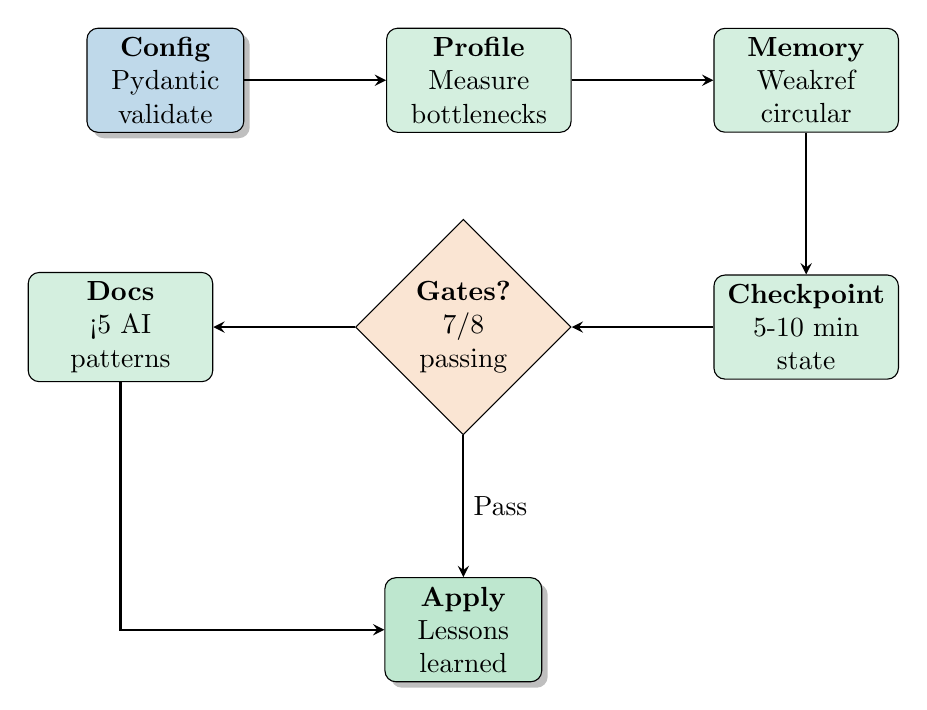
\begin{tikzpicture}[node distance=1.8cm, auto]
    \node[block, fill=primary!30] (config) {\textbf{Config}\\Pydantic\\validate};
    \node[process, right=of config] (profile) {\textbf{Profile}\\Measure\\bottlenecks};
    \node[process, right=of profile] (memory) {\textbf{Memory}\\Weakref\\circular};
    \node[process, below=of memory] (checkpoint) {\textbf{Checkpoint}\\5-10 min\\state};
    \node[decision, left=of checkpoint] (gates) {\textbf{Gates?}\\7/8\\passing};
    \node[process, left=of gates] (docs) {\textbf{Docs}\\<5 AI\\patterns};
    \node[block, fill=secondary!30, below=of gates] (apply) {\textbf{Apply}\\Lessons\\learned};

    \draw[arrow] (config) -- (profile);
    \draw[arrow] (profile) -- (memory);
    \draw[arrow] (memory) -- (checkpoint);
    \draw[arrow] (checkpoint) -- (gates);
    \draw[arrow] (gates) -- (docs);
    \draw[arrow] (docs) |- (apply);
    \draw[arrow] (gates) -- node[right] {Pass} (apply);
\end{tikzpicture}
\end{center}

\begin{itemize}
  \item[$\square$] \textbf{Config Validation}: Use Pydantic or similar (fail fast at load time)
  \item[$\square$] \textbf{Profile Before Optimizing}: Measure bottlenecks, don't guess
  \item[$\square$] \textbf{Memory Management}: Check for circular refs (use weakref where needed)
  \item[$\square$] \textbf{Checkpoint Long Tasks}: Save state every 5-10 min (assume interruptions)
  \item[$\square$] \textbf{Quality Gates}: Automate 7+/8 in pre-commit hooks
  \item[$\square$] \textbf{Documentation Standards}: Scan for AI-ish patterns (<5 per file)
  \item[$\square$] \textbf{3-Tier Coverage}: Set targets (85\%/95\%/100\% for overall/critical/safety)
  \item[$\square$] \textbf{Intentional Patterns}: Document architectural decisions (prevent future "fixes")
\end{itemize}

% =============================================================================
% NEXT STEPS
% =============================================================================
\section*{Next Steps}
\begin{itemize}
  \item \textbf{E025-E029}: Appendix reference (5-part technical deep dive)
  \item \textbf{Apply Lessons}: Use these patterns in your own projects
  \item \textbf{Contribute}: Share improvements to DIP-SMC-PSO (post-publication)
\end{itemize}

\end{document}
